\documentclass{tietreport}

% Import images
\usepackage{graphicx}
\usepackage[T1]{fontenc}

% Diagrams: use case, class, sequence and activity diagrams are all
% drawn natively in TikZ (no external image files needed).
\usepackage{tikz}
\usetikzlibrary{shapes.geometric, shapes.multipart, arrows.meta, positioning, calc, fit, backgrounds}

\tikzset{
  actorlbl/.style={font=\scriptsize\bfseries, align=center},
  usecase/.style={ellipse, draw=black!70, fill=blue!6, minimum width=30mm,
                   minimum height=9mm, align=center, font=\scriptsize, inner sep=1pt},
  sysbound/.style={rectangle, rounded corners=3pt, draw=black!60, thick, inner sep=8mm},
  relarr/.style={draw=black!70},
  incarr/.style={draw=black!60, dashed, -{Latex[length=1.8mm]}},
  umlclass/.style={rectangle split, rectangle split parts=3, draw=black!70,
                    fill=green!5, font=\tiny, text width=30mm,
                    rectangle split part align=left, align=left, inner sep=1.5mm},
  gen/.style={-{Triangle[open, length=2.4mm, width=2mm]}, draw=black!70},
  lifeline/.style={draw=black!60, dash pattern=on 2pt off 2pt},
  seqhead/.style={rectangle, draw=black!70, fill=blue!8, minimum width=30mm,
                  minimum height=8mm, align=center, font=\scriptsize},
  actbar/.style={rectangle, draw=black!70, fill=gray!15},
  seqmsg/.style={-{Latex[length=2.2mm]}, draw=black!80, font=\tiny},
  seqret/.style={-{Latex[length=2.2mm]}, draw=black!55, dashed, font=\tiny},
  seqframe/.style={rectangle, draw=black!55, dashed, inner sep=0pt},
  seqtab/.style={rectangle, draw=black!55, fill=white, font=\tiny\bfseries, inner sep=1.5pt, anchor=north west},
  lanehdr/.style={rectangle, draw=black!70, fill=black!8, minimum width=48mm,
                  minimum height=7mm, align=center, font=\scriptsize\bfseries},
  swimsep/.style={draw=black!45},
  actn/.style={rectangle, rounded corners=2pt, draw=black!70, fill=blue!6,
               minimum height=9mm, text width=40mm, align=center, font=\scriptsize},
  actnb/.style={actn, text width=30mm},
  actdecw/.style={diamond, aspect=2.4, draw=black!70, fill=orange!10,
                  font=\scriptsize, align=center, inner sep=1pt, text width=26mm},
  actend/.style={circle, draw=black!80, fill=white, minimum size=5mm},
  actflow/.style={-{Latex[length=2mm]}, draw=black!75},
}
\newcommand{\stickactor}[4]{%
  \begin{scope}[shift={(#1,#2)}]
    \node[rectangle, minimum width=9mm, minimum height=16mm, inner sep=0pt,
          draw=none, fill=none] (#3) {};
    \draw[thick] (0,0.95) circle (0.16);
    \draw[thick] (0,0.79) -- (0,0.15);
    \draw[thick] (-0.26,0.6) -- (0.26,0.6);
    \draw[thick] (0,0.15) -- (-0.22,-0.25);
    \draw[thick] (0,0.15) -- (0.22,-0.25);
    \node[actorlbl] at (0,-0.55) {#4};
  \end{scope}%
}
\newcommand{\rel}[3]{\draw[incarr] (#1) -- node[font=\tiny,fill=white,inner sep=1pt,pos=0.5]{\guillemotleft#2\guillemotright} (#3);}
\newcommand{\startnode}[1]{\node[circle,draw=black,fill=black,minimum size=3.6mm] #1 {};}
\newcommand{\actendnode}[2]{\node[actend] (#1) #2 {}; \node[circle,draw=black,fill=black,minimum size=2.6mm] at (#1) {};}

% Bibliography configuration
\usepackage[
  date=year,
  style=alphabetic,
  backend=biber,
  sorting=nty,
  maxnames=5,
  minnames=3,
  maxalphanames=4,
  minalphanames=3,
  backref=true,
  doi=false,
  isbn=false,
  url=false,
  eprint=false
]{biblatex}
\addbibresource{references.bib}

%% ==================================================
%% PROJECT FIELDS
%% ==================================================

\TitlePageHeader{%
  UCS503 -- Software Engineering Lab%
}

\ProjectTitle{%
  SHARP: A Smart Hostel Administration and Resource Platform%
}

\ProjectSubTitle{%
  Use Case and UML Design for Digital Hostel Workflows%
}

\author{%
  \texttt{1024160097} Vaibhav Kansal \\
  \texttt{1024160138} Ali Ekram \\
  \texttt{1024160122} Riya Gupta \\
  \texttt{1024160118} Ayush Kamboj%
}

\TitlePageSubText{%
  Group: \texttt{3P14}, BE Third Year, CSE%
}

\AdvisorName{%
  Ms. Anushka%
}

\TitlePageFooterText{{%
    \large PROJECT REPORT \\[0.2cm]
    \bfseries Computer Science and Engineering
    Department%
  } \\[0.15cm]
  Thapar Institute of Engineering and Technology,
  Patiala%
}

%% ==================================================

\begin{document}

\maketitle
\tableofcontents

% =====================================================================
\chapter{Introduction}

\section{Background and Context}

Hostel administration at Thapar Institute of Engineering and Technology
currently depends on a mix of handwritten applications, physical registers,
and informally tracked complaints spread across five recurring processes:
leave and visitor passes, mess feedback, room allotment, maintenance
complaints, and laundry issue reporting. None of these processes currently
produce an auditable digital record, which makes it difficult to measure
resolution time, detect recurring problems, or settle disputes between
students and hostel staff.

SHARP (Smart Hostel Administration and Resource Platform) is proposed as a
single web-based system that converts these five processes into structured,
traceable digital workflows. The immediate engineering objective is not
novel algorithm research but \emph{reliable, verifiable service delivery}:
every request should carry a unique identifier, a defined owner, and a
timestamped history from creation to closure. The system is intended to
scale from a single pilot hostel wing to the full campus without a
redesign, by keeping each of the five service modules independent behind a
common authentication and role-based access layer.

\subsection{Problem Statement}

Five specific pain points motivate the system:

\begin{itemize}
  \item \textbf{Leave and passes:} paper applications and manual parent
    contact create delay and are easy to lose or misrepresent.
  \item \textbf{Mess feedback:} register-based feedback is visible to mess
    staff, which discourages honest reporting.
  \item \textbf{Allotment:} when members of the same room cluster pay at
    different times, a partially reserved room can be taken by someone
    else, breaking up the cluster.
  \item \textbf{Maintenance:} complaints have no owner or deadline once
    filed, so resolution time and preferred repair slots go untracked.
  \item \textbf{Laundry:} damaged or missing items are reported informally,
    so recurring problems by day, batch, or item type go unnoticed.
\end{itemize}

Because hostel staff bandwidth is limited relative to the student
population, even small structural improvements -- a unique complaint ID,
an allotment expiry rule, a Service Level Agreement (SLA) timer -- are
expected to measurably reduce unresolved cases and disputes.

\section{Project Objectives}

\begin{enumerate}
  \item \textbf{Role-based access first:} deliver authentication and
    role-based access control for all six user roles (Student, Parent,
    Warden, Caretaker, Mess Staff, Laundry Staff) before any service
    module, so every subsequent workflow is access-controlled from the
    start.
  \item \textbf{Leave workflow as first vertical slice:} implement the
    leave and visitor pass workflow end to end (Student
    $\rightarrow$ Parent verification $\rightarrow$ Warden approval
    $\rightarrow$ digital pass) as the first complete, demonstrable path
    through the system.
  \item \textbf{Complaint lifecycle as second vertical slice:} implement
    complaint filing, caretaker assignment, SLA-timed escalation, and
    student-verified closure, since this workflow is the primary source
    of the project's evaluation metrics.
  \item \textbf{Model before building:} fix the user/functionality
    boundary with a use case diagram, and fix the data model and two
    representative workflows with UML class, sequence, and activity
    diagrams, before implementation of each module begins.
  \item \textbf{Independent, deployable modules:} design every module so
    the mess, allotment, and laundry modules can be added in later
    iterations without redesigning the authentication, complaint, or
    leave modules already in place.
\end{enumerate}

Objectives 1--3 are Specific, Measurable (each has a clear
done/not-done boundary), Achievable within a lab-scale project,
Relevant to the problem statement above, and Time-bound by the phased
delivery plan in Section~\ref{sec:modules}.

% =====================================================================
\chapter{Methodology and Design}
\label{ch:design}

\section{System Architecture}

\subsection{High-Level Design}

SHARP follows a five-tier layered architecture rather than a monolithic
design, so that any one concern can change without forcing a redesign of
the others:

\begin{itemize}
  \item \textbf{Interface layer:} role-specific portals for
    students/parents, wardens/admins, and caretaker/mess/laundry staff.
  \item \textbf{Application layer:} REST API endpoints, authentication
    (hashed credentials, tokens), and role-based access control.
  \item \textbf{Application services layer:} the five service modules
    (leave \& pass, mess feedback, allotment, complaints \& SLA, laundry
    issues) plus notifications and analytics.
  \item \textbf{Data layer:} users, requests, complaints and reports,
    status history, audit records, backup and recovery.
  \item \textbf{External services layer (optional):} email, SMS, or push
    notification providers.
\end{itemize}

Every sensitive endpoint checks both identity and permission, so, for
example, a student cannot reach warden dashboards, parent contact records,
or the identity behind an anonymous mess feedback entry.

\subsection{Technical Stack}

The layers above are specified by responsibility rather than by product,
so the exact implementation stack is finalised at build time. The current
working assumption is:

\begin{itemize}
  \item \textbf{Frontend:} React with Tailwind CSS for role-specific
    reactive pages.
  \item \textbf{Backend:} Node.js with Express.
  \item \textbf{Database:} MongoDB.
  \item \textbf{Authentication:} token-based authentication with hashed
    credentials.
  \item \textbf{Testing:} a unit/integration test framework exercised on
    every change.
  \item \textbf{CI/CD:} a CI runner with staging deployment.
\end{itemize}

No workflow rule, role definition, or evaluation metric in this report
depends on this specific stack, so deferring the final choice costs
nothing structurally.

\section{System Users and Use Cases}
\label{sec:actors}

Six users interact with SHARP. Table~\ref{tab:actors} identifies each
user and the use cases it participates in; these are the same use cases
drawn in Figure~\ref{fig:usecase}.

\begin{table}[h]
\centering
\small
\begin{tabular}{|l|p{3.6cm}|p{6.6cm}|}
  \hline
  \textbf{User} & \textbf{Role} & \textbf{Primary Use Cases} \\
  \hline
  Student & Primary end user; a hostel resident & Login/Authenticate, Apply
    for Leave/Pass, Submit Mess Feedback, Request Room Allotment, Make
    Payment, File Complaint, Verify Complaint Resolution, Report Laundry
    Issue, Track Request Status \\
  \hline
  Parent & Secondary human user; verifies a leave request for their
    child & Verify Leave Request \\
  \hline
  Warden & Hostel administrator for a block & Approve Leave Request,
    Assign Caretaker, Handle SLA Escalation, View Analytics Dashboard \\
  \hline
  Caretaker & Maintenance staff & Update Complaint Status \\
  \hline
  Mess Staff & Mess operations staff & View Aggregated Mess Feedback \\
  \hline
  Laundry Staff & Laundry operations staff & Update Laundry Issue Status \\
  \hline
\end{tabular}
\caption{Users and their primary use cases}
\label{tab:actors}
\end{table}

\section{Use Case Diagram}

Figure~\ref{fig:usecase} follows the OMG UML 2.5.1
notation~\cite{umlspec}: users are drawn outside the system boundary,
use cases are ellipses inside it, and \guillemotleft
include\guillemotright/\guillemotleft extend\guillemotright\ dependencies
capture mandatory and optional sub-behaviour. Three relationships are
worth calling out explicitly, since they encode workflow rules from
Section~\ref{sec:actors} directly into the model:

\begin{itemize}
  \item \emph{Apply for Leave/Pass} includes \emph{Verify Leave Request},
    which itself includes \emph{Approve Leave Request} -- the same
    three-step approval chain (Student $\rightarrow$ Parent
    $\rightarrow$ Warden) described in Section~\ref{sec:modules}.
  \item \emph{File Complaint} includes \emph{Assign Caretaker} (assignment
    is mandatory on every complaint) but is only \emph{extended} by
    \emph{Handle SLA Escalation}, since escalation is conditional on the
    SLA timer actually being breached.
  \item \emph{Request Room Allotment} includes \emph{Make Payment}, since
    a cluster reservation is not confirmed until payment completes.
\end{itemize}

\emph{Login/Authenticate} is included by every primary student
transaction; only one representative edge is drawn in the diagram to keep
it legible.

\begin{figure}[p]
\centering
\resizebox{\linewidth}{!}{%
\begin{tikzpicture}[node distance=6mm, >=Latex]

\node[sysbound, minimum width=96mm, minimum height=199mm] (sys) at (5.3,-8.65) {};
\node[font=\scriptsize\bfseries] at (5.3,1.7) {SHARP: Hostel Administration System};

\node[usecase] (uc1)  at (1.9,  0.0) {Login /\\Authenticate};
\node[usecase] (uc2)  at (1.9, -2.2) {Apply for\\Leave / Pass};
\node[usecase] (uc3)  at (1.9, -4.4) {Submit Mess\\Feedback};
\node[usecase] (uc4)  at (1.9, -6.6) {Request Room\\Allotment};
\node[usecase] (uc5)  at (1.9, -8.8) {Make\\Payment};
\node[usecase] (uc6)  at (1.9,-11.0) {File\\Complaint};
\node[usecase] (uc7)  at (1.9,-13.2) {Verify Complaint\\Resolution};
\node[usecase] (uc8)  at (1.9,-15.4) {Report Laundry\\Issue};
\node[usecase] (uc9)  at (1.9,-17.2) {Track Request\\Status};

\node[usecase] (uc10) at (8.7, -2.2) {Verify Leave\\Request};
\node[usecase] (uc11) at (8.7, -4.6) {Approve Leave\\Request};
\node[usecase] (uc12) at (8.7, -6.6) {Assign\\Caretaker};
\node[usecase] (uc14) at (8.7, -8.8) {Handle SLA\\Escalation};
\node[usecase] (uc17) at (8.7,-11.0) {View Analytics\\Dashboard};
\node[usecase] (uc13) at (8.7,-13.2) {Update Complaint\\Status};
\node[usecase] (uc15) at (8.7,-15.2) {View Aggregated\\Mess Feedback};
\node[usecase] (uc16) at (8.7,-17.0) {Update Laundry\\Issue Status};

\stickactor{-1.9}{-5.0}{actStudent}{Student}

\stickactor{12.0}{-2.2}{actParent}{Parent}
\stickactor{12.0}{-7.5}{actWarden}{Warden}
\stickactor{12.0}{-13.2}{actCaretaker}{Caretaker}
\stickactor{12.0}{-15.1}{actMess}{Mess Staff}
\stickactor{12.0}{-17.3}{actLaundry}{Laundry Staff}

\foreach \i in {1,2,3,4,6,7,8,9}{
  \draw[relarr] (actStudent) -- (uc\i);
}

\draw[relarr] (actParent) -- (uc10);

\draw[relarr] (actWarden) -- (uc11);
\draw[relarr] (actWarden) -- (uc12);
\draw[relarr] (actWarden) -- (uc14);
\draw[relarr] (actWarden) -- (uc17);

\draw[relarr] (actCaretaker) -- (uc13);
\draw[relarr] (actMess) -- (uc15);
\draw[relarr] (actLaundry) -- (uc16);

\rel{uc2}{include}{uc1}
\rel{uc2}{include}{uc10}
\rel{uc10}{include}{uc11}
\rel{uc4}{include}{uc5}
\rel{uc6}{include}{uc12}
\rel{uc6}{extend}{uc14}

\node[font=\tiny, align=left, text width=90mm] at (5.3,-20.0)
 {\guillemotleft include\guillemotright\ \emph{Login/Authenticate} is included by every
 primary transaction (Apply for Leave, Mess Feedback, Allotment, Complaint,
 Laundry Issue); only one representative edge is drawn above for legibility.};

\end{tikzpicture}}
\caption{Use Case Diagram: SHARP Hostel Administration System}
\label{fig:usecase}
\end{figure}

\section{Class Diagram}

Figure~\ref{fig:class} is the class diagram produced for SHARP's domain
model. \texttt{User} is an abstract base class carrying shared
authentication attributes (\texttt{userId}, \texttt{name},
\texttt{email}, \texttt{password}) and behaviour (\texttt{login()},
\texttt{logout()}); the six user roles are modelled as subclasses
connected to \texttt{User} by generalization (hollow-triangle arrows).
Each role carries only the attributes and methods specific to it --
for example \texttt{Warden} adds \texttt{approveLeave()},
\texttt{manageAllotment()}, \texttt{monitorSLA()}, and
\texttt{viewReports()}, while \texttt{Caretaker} adds
\texttt{manageComplaint()} and \texttt{updateRepairStatus()}.

Below the user layer, the diagram groups the domain classes into the
five service modules from Section~\ref{sec:modules}: \emph{Leave
Management} (\texttt{LeaveRequest}, which generates at most one
\texttt{DigitalPass} once both \texttt{parentVerified} and
\texttt{wardenApproved} are true -- a 1..0..1 association),
\emph{Maintenance Management} (\texttt{Complaint}, with
\texttt{slaDeadline} and \texttt{create()}/\texttt{assign()}/
\texttt{updateStatus()}/\texttt{verifyResolution()}/\texttt{close()}/
\texttt{reopen()}), \emph{Room Allotment} (\texttt{RoomReservation},
with \texttt{reserve()}/\texttt{confirm()}/\texttt{expire()}
implementing the cluster-expiry rule from the proposal),
\emph{Mess Management} (\texttt{MessFeedback}), and \emph{Laundry
Management} (\texttt{LaundryIssue}). \texttt{Student} is associated
1..0..* with all five module classes, since a student is the one user
who creates every kind of request; \texttt{Parent} and \texttt{Warden}
are associated with \emph{Leave Management} (verifying and approving a
\texttt{LeaveRequest} respectively); \texttt{Warden} and
\texttt{Caretaker} are both associated with \emph{Maintenance
Management}, matching \texttt{monitorSLA()} and
\texttt{manageComplaint()}; and \texttt{MessStaff}/\texttt{LaundryStaff}
are associated with their respective modules only.

\begin{figure}[p]
\centering
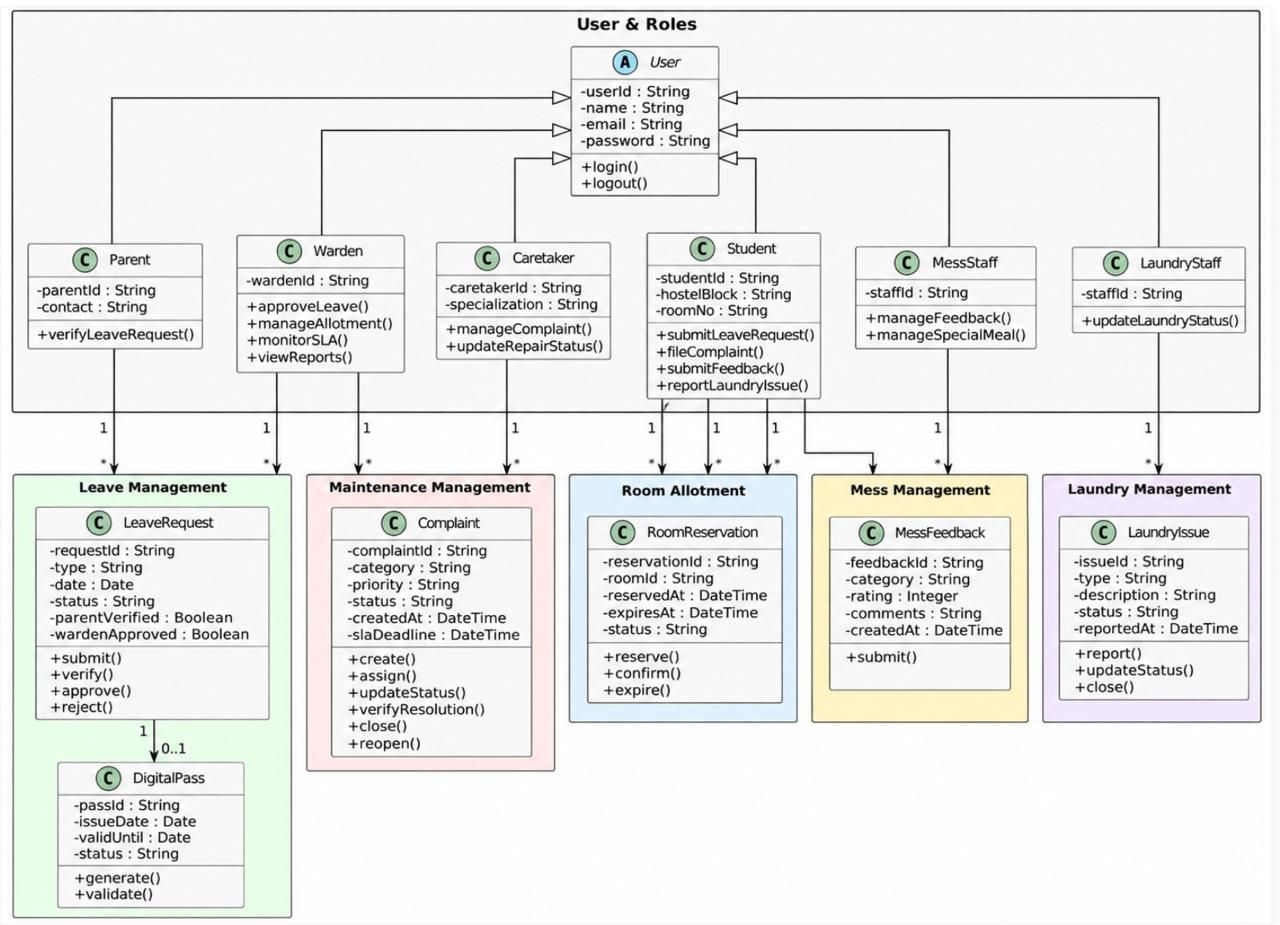
\includegraphics[width=\linewidth]{assets/class_diagram.jpg}
\caption{Class Diagram: SHARP core domain model}
\label{fig:class}
\end{figure}

\section{Sequence Diagram: Complaint Lifecycle}

Figure~\ref{fig:sequence} traces the complaint lifecycle as message
exchanges among five lifelines: the \texttt{Student}, \texttt{Caretaker}
and \texttt{Warden} users, the \texttt{SHARP System} that mediates
every request, and the \texttt{Complaint Database} it persists to.
The system, not the users, owns every write to the database: a
complaint record is created and given an ID as soon as it is filed, the
caretaker's repair status is saved as it changes, and the closing or
reopening of a complaint is itself a database write triggered by the
system after the student's verification message. Two \texttt{alt}
frames capture the workflow's two decision points -- whether the
student verifies the resolution (closing or reopening the same
complaint ID) -- while a second, independent \texttt{alt}\ [SLA
breached] frame sends an escalation notification to the Warden without
being on the critical path of the student-facing flow at all. This
matches the closure rule in Section~\ref{sec:modules}: a failed
verification reopens the existing complaint rather than creating a new
one.

\begin{figure}[p]
\centering
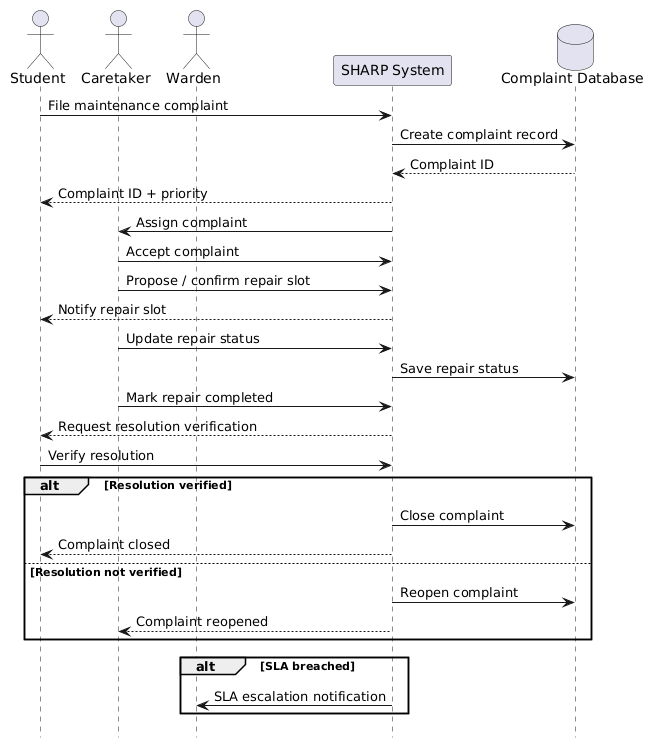
\includegraphics[width=0.92\linewidth]{assets/sequence_diagram.png}
\caption{Sequence Diagram: Complaint Lifecycle}
\label{fig:sequence}
\end{figure}

\section{Activity Diagram: Complaint Lifecycle}

Where Figure~\ref{fig:sequence} shows the complaint lifecycle as
messages between users and the system, Figure~\ref{fig:activity} shows
the same lifecycle as a single control flow, which is the clearer view
of the two decision points once who-sends-what stops being the
question. After a complaint is filed, its ID and priority are generated
and a caretaker is assigned automatically. The first decision, `Repair
slot agreed?', has both branches -- accepting the proposed slot, or the
caretaker proposing an alternative -- merge back into a single `Repair
completed' step, since the diagram treats slot negotiation as a detail
that does not change what happens next. The second decision, `Resolution
verified?', closes or reopens the complaint. Only after that merge does
the diagram check `SLA breached?': this ordering places the SLA check
after resolution rather than racing it against the main flow, which is
a simpler model than the sequence diagram's independent \texttt{alt}
frame, at the cost of not showing that the SLA timer can in practice
breach and notify the Warden \emph{before} the complaint is resolved.
The two diagrams are deliberately kept as complementary views rather
than reconciled into one, since each makes a different property of the
workflow easier to see.

\begin{figure}[p]
\centering
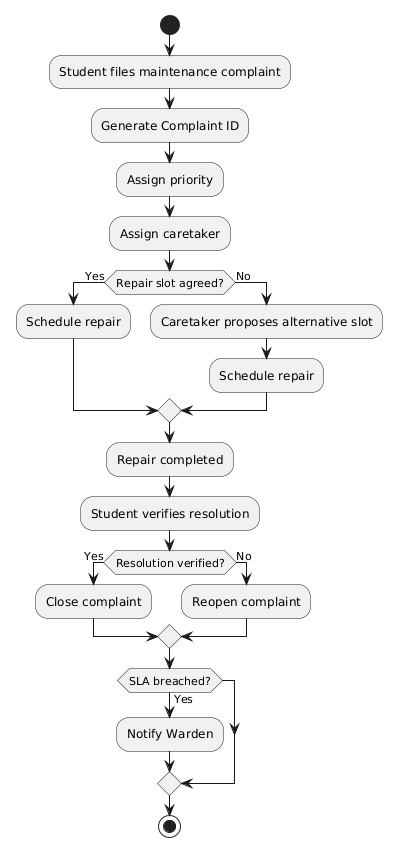
\includegraphics[width=0.55\linewidth]{assets/activity_diagram.png}
\caption{Activity Diagram: Complaint Lifecycle}
\label{fig:activity}
\end{figure}

\section{Implementation Modules}
\label{sec:modules}

The four diagrams above cover the full system, but delivery is phased.
The initial deliverable is:

\begin{itemize}
  \item Authentication and role-based access control for all six roles.
  \item The leave and visitor pass workflow (Student $\rightarrow$
    Parent $\rightarrow$ Warden $\rightarrow$ digital pass).
  \item The complaint lifecycle (filing, assignment, SLA timer, verified
    closure) -- modelled in Figure~\ref{fig:sequence}.
  \item Basic logging and timestamps to support the resolution-time
    metric in Section~\ref{sec:metrics}.
  \item CI: build, backend unit tests, and linting on every change.
  \item CD to a staging environment from a single pipeline job.
\end{itemize}

Subsequent deliverables, built on the same class model
(Figure~\ref{fig:class}) and layered architecture, are the mess feedback
module (anonymous to staff, with internal abuse-deterrence records), the
allotment module (temporary reservation with expiry), laundry issue
tracking with recurring-issue aggregation, an in-app notification layer,
and a warden/admin analytics dashboard.

\section{Risk Management}

Risks were identified against the design in this chapter rather than
left for the implementation phase:

\begin{itemize}
  \item \textbf{Unauthorised access} is mitigated by the role-based
    access control enforced at the application layer for every request.
  \item \textbf{Forged parent approval} is mitigated by secure,
    single-use verification tokens combined with a subsequent warden
    check, rather than relying on parent verification alone.
  \item \textbf{Abuse of anonymous mess feedback} is mitigated by rate
    limits and an internal audit trail that is not exposed to mess staff.
  \item \textbf{Premature loss of a room reservation} is mitigated by the
    \texttt{Allotment} class's expiry rule and transactional payment
    validation.
  \item \textbf{Disputed laundry loss} is mitigated by timestamped
    \texttt{LaundryIssue} reports tied to a specific submission.
\end{itemize}

\section{Prototype}
\label{sec:prototype}

A working prototype of SHARP has been built to check the design above
against a real interface, currently covering the debug/demo
authentication flow and both the caretaker- and student-facing sides of
the room allocation console for Phase 2 (Cluster Formation) of the
allotment module. Figure~\ref{fig:proto-home} shows the landing page: a
demo role switcher bypasses manual login for testing, and the page
reports campus-wide capacity figures (11 hostels, 8 floors per hostel,
50 rooms per floor, 8,800 total bed capacity) that the schema in
Figure~\ref{fig:class} is sized against.

On the caretaker side, Figure~\ref{fig:proto-dashboard} shows the
caretaker's dashboard scoped to a single assigned facility (Hostel M,
Anantam Hall), consistent with the role-based access rule in
Section~2.1.1: a caretaker sees only the hostel block they are assigned
to, not the full campus. Figure~\ref{fig:proto-allocation} shows the
caretaker's room allocation console: each candidate cluster lists its
members by roll number, average CGPA, eligible hostels in preference
order, and a status of \texttt{FORMED}, \texttt{ALLOCATED}, or
\texttt{CONFIRMED} -- a direct implementation of the cluster-preservation
rule from the original problem statement, where a cluster is only
finalised once every member's preferences and payment status agree,
rather than allocating rooms to individual students as they pay.

On the student side, Figure~\ref{fig:proto-student} shows the same
role-scoped pattern from the other direction: a student sees only their
own room, resident ID, and allocation status, with room allocation and
room/hostel info as the only two actions exposed for this phase.
Figure~\ref{fig:proto-student-allocation} shows what a cluster leader
sees when they open that action: the same cluster (members, average
CGPA, eligible hostels) the caretaker sees in
Figure~\ref{fig:proto-allocation}, but from the student's side, with
controls to submit room-pair preferences or change the cluster leader
rather than to allocate or resolve conflicts. Together the two pairs of
screens show the same \texttt{RoomReservation} data
(Figure~\ref{fig:class}) correctly restricted to what each role is
allowed to do with it.

This prototype currently demonstrates the \texttt{RoomReservation}
portion of the class diagram (Figure~\ref{fig:class}); the leave and
complaint vertical slices described in Section~\ref{sec:modules} are
the next modules to be connected to a similar interface.

\begin{figure}[h]
\centering
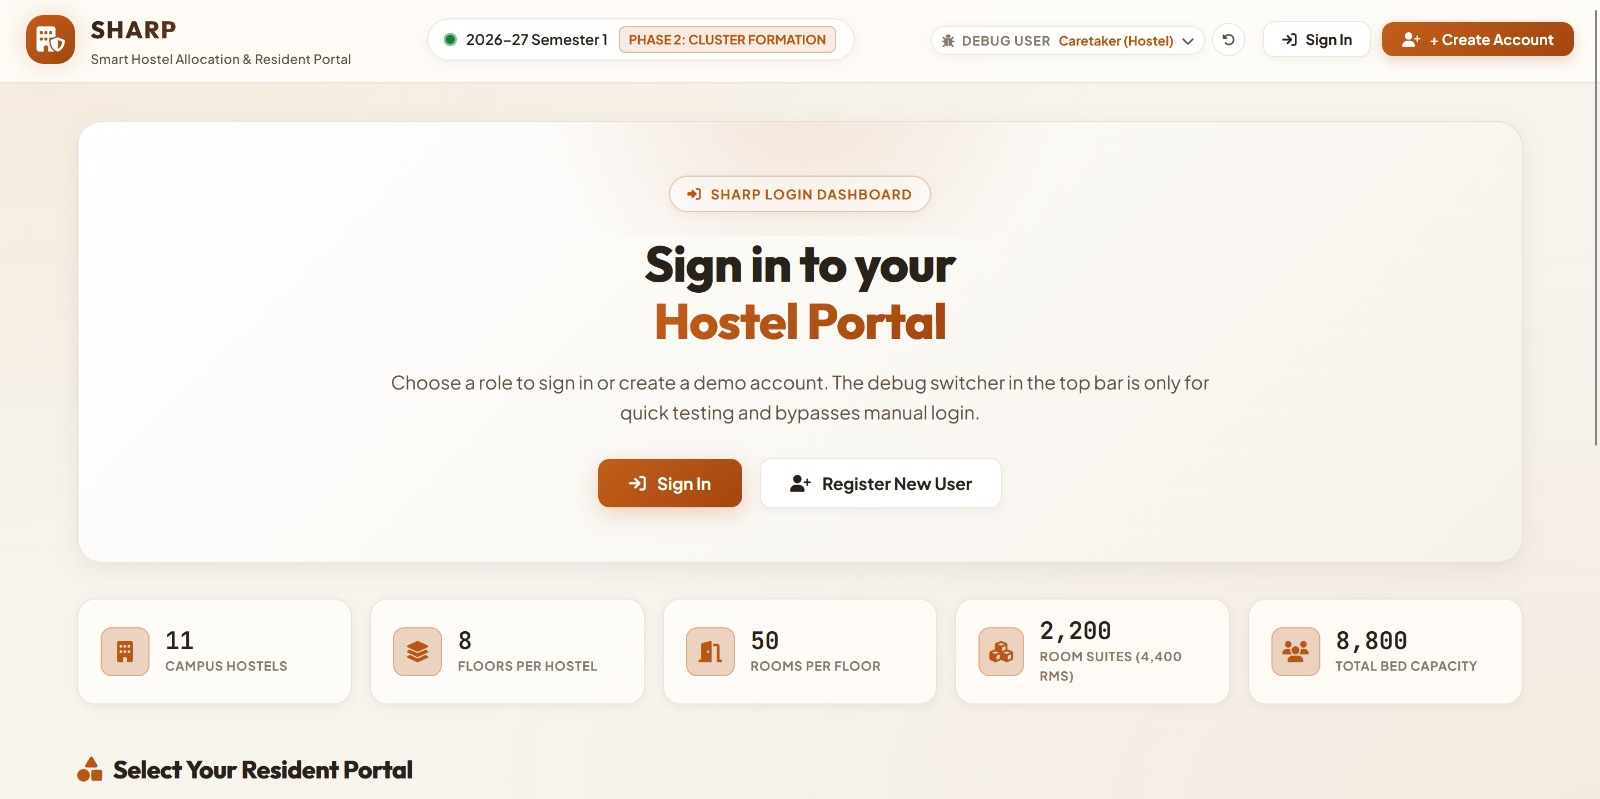
\includegraphics[width=0.95\linewidth]{assets/proto_home.jpg}
\caption{Prototype: landing page and role selection}
\label{fig:proto-home}
\end{figure}

\begin{figure}[h]
\centering
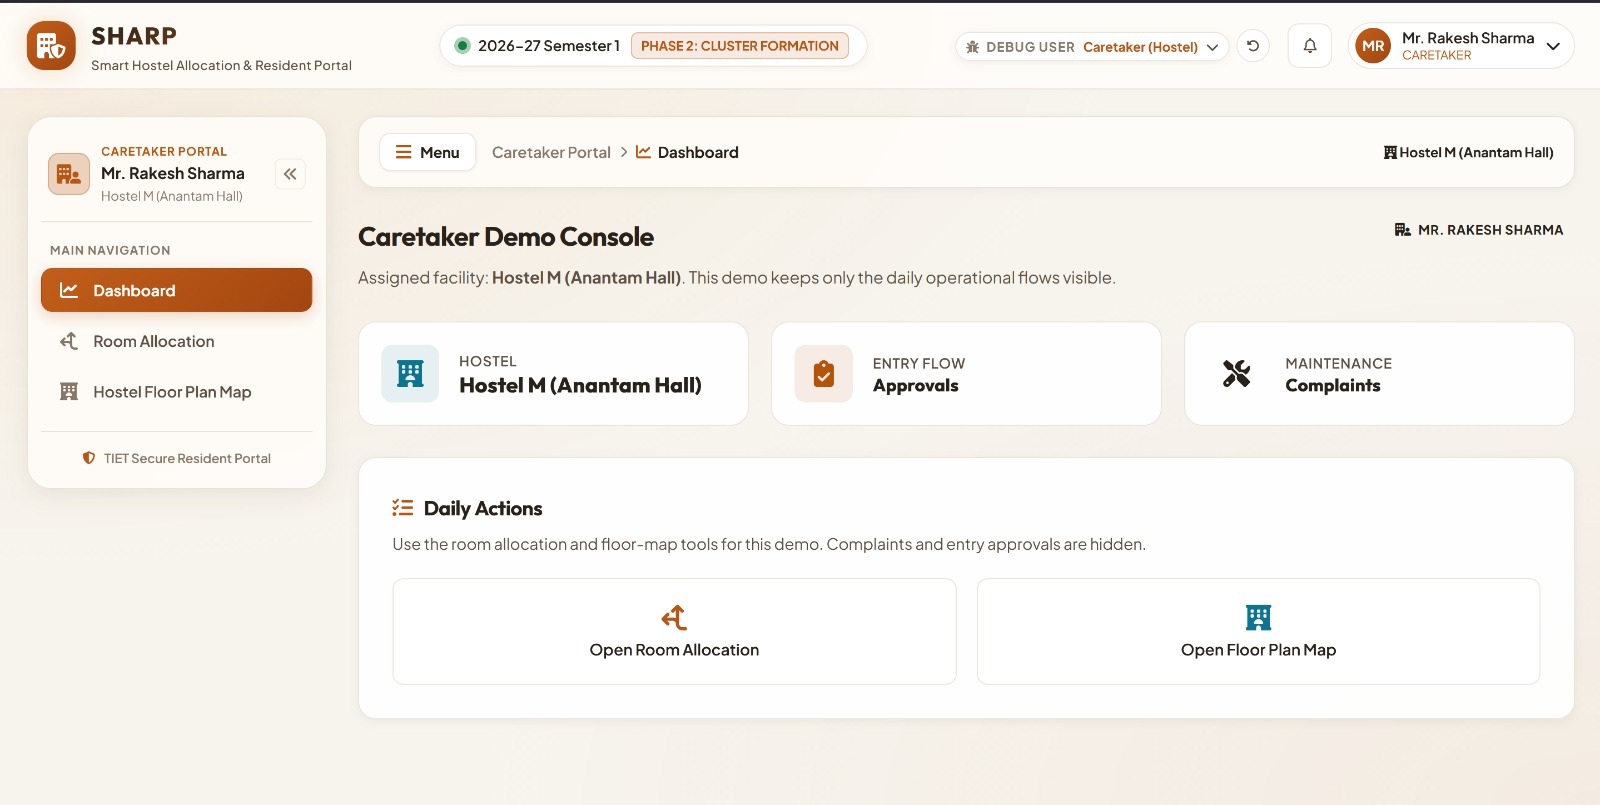
\includegraphics[width=0.95\linewidth]{assets/proto_dashboard.jpg}
\caption{Prototype: caretaker dashboard, scoped to one hostel block}
\label{fig:proto-dashboard}
\end{figure}

\begin{figure}[h]
\centering
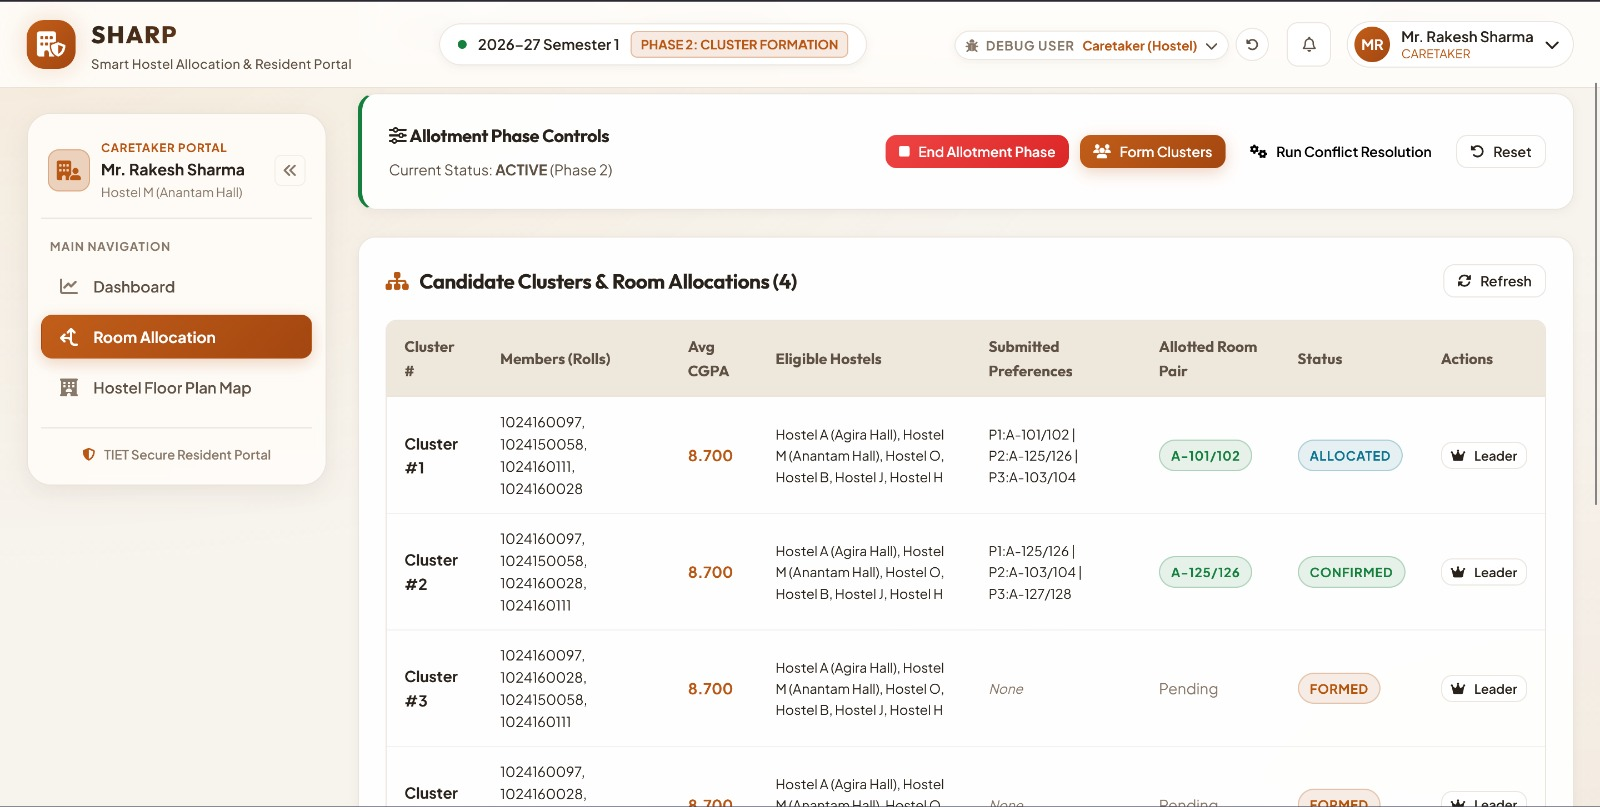
\includegraphics[width=0.95\linewidth]{assets/proto_allocation.jpg}
\caption{Prototype: caretaker's room allocation and cluster formation console}
\label{fig:proto-allocation}
\end{figure}

\begin{figure}[h]
\centering
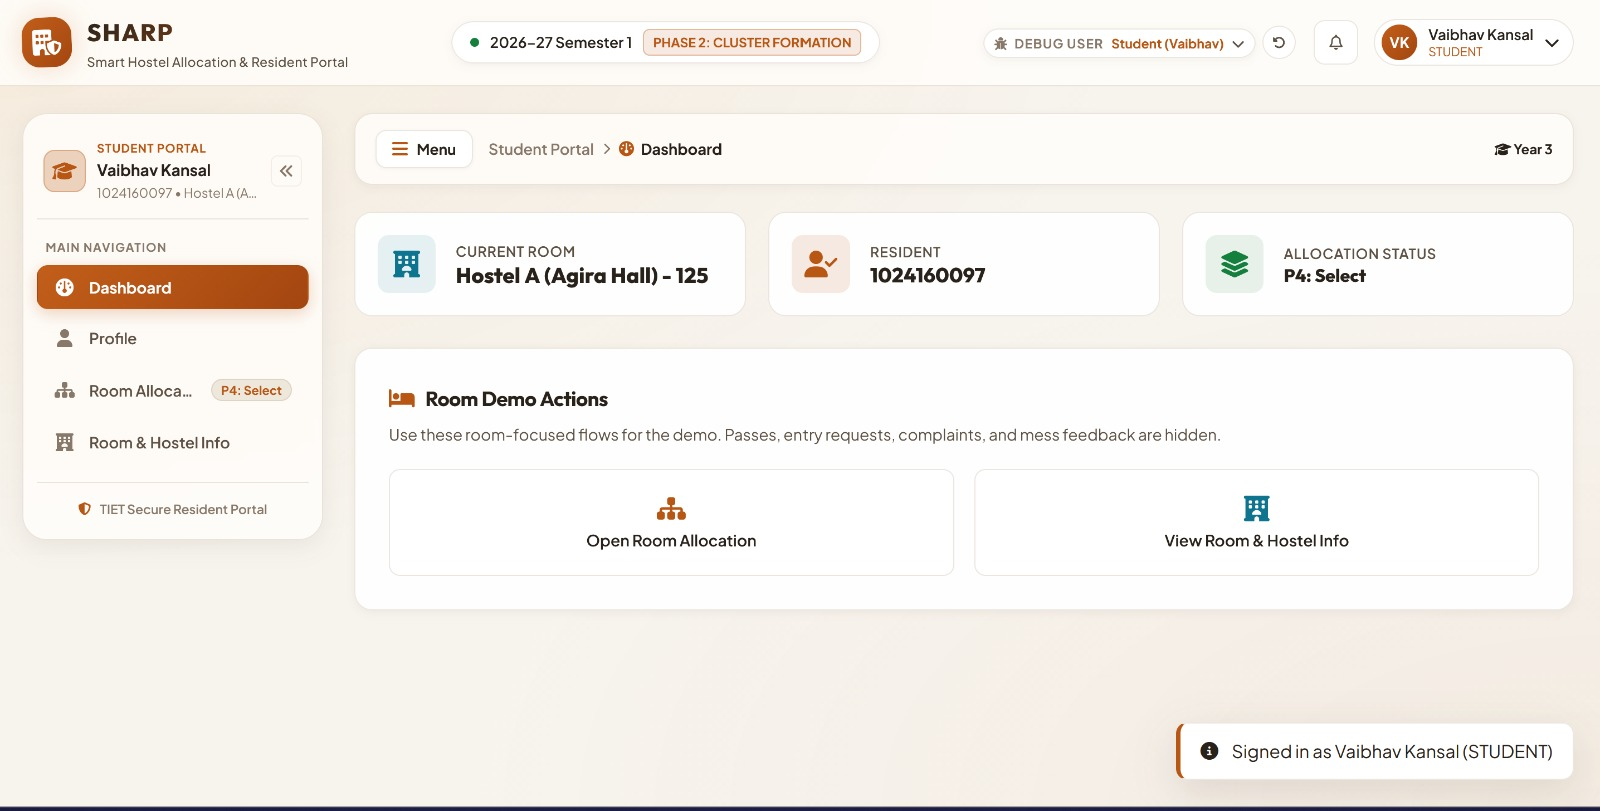
\includegraphics[width=0.95\linewidth]{assets/proto_student.jpg}
\caption{Prototype: student dashboard, scoped to one resident}
\label{fig:proto-student}
\end{figure}

\begin{figure}[h]
\centering
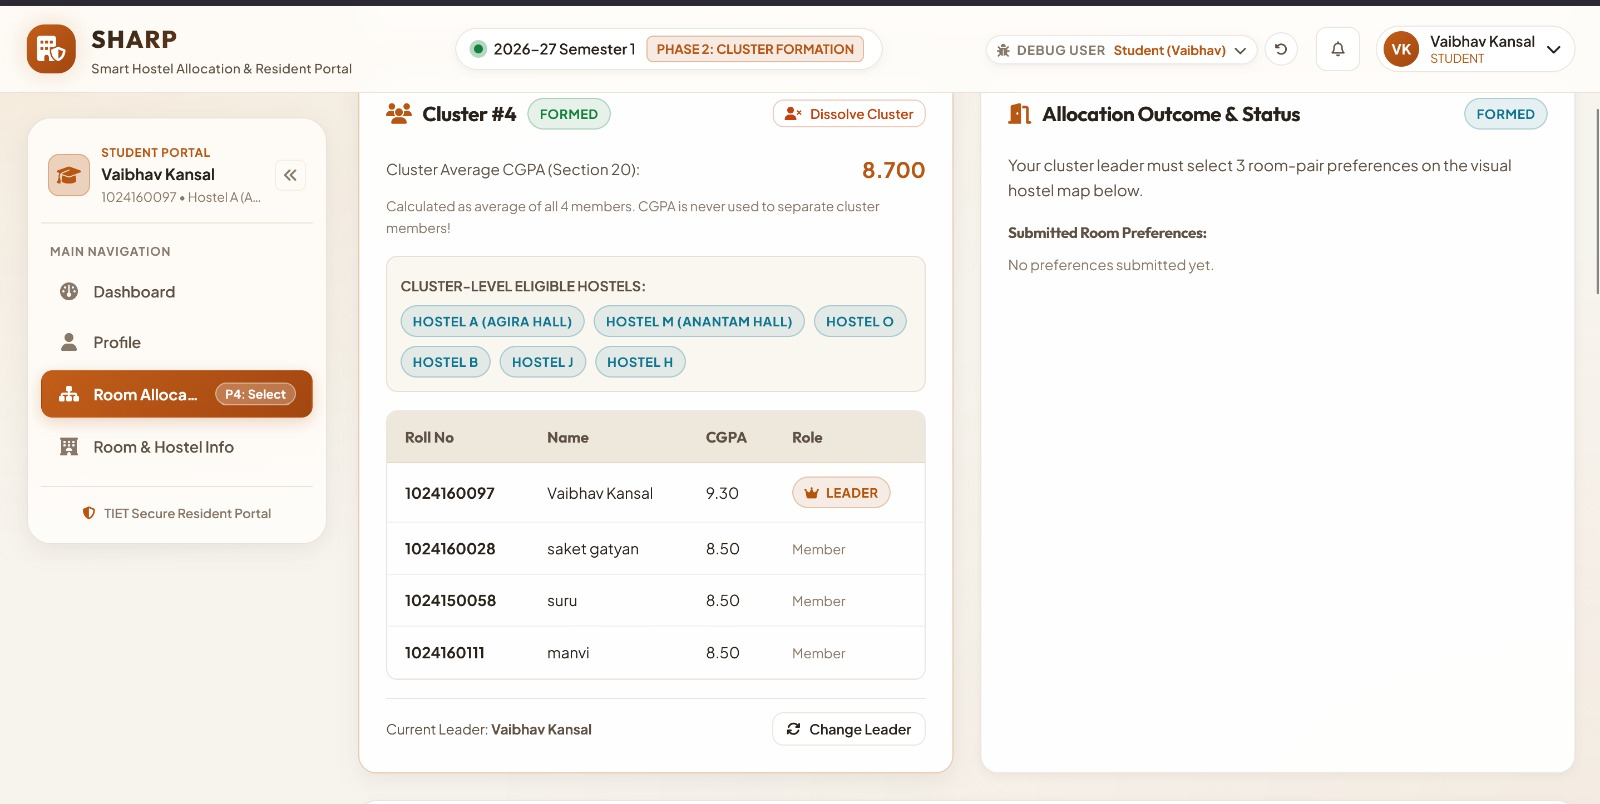
\includegraphics[width=0.95\linewidth]{assets/proto_student_allocation.jpg}
\caption{Prototype: student-facing cluster and room preference view}
\label{fig:proto-student-allocation}
\end{figure}

% =====================================================================
\chapter{Results and Evaluation}

This report documents SHARP partway between design and implementation:
the use case and UML diagrams in Chapter~\ref{ch:design} are complete,
and a first prototype (Section~\ref{sec:prototype}) demonstrates the
room allocation console end to end. The leave and complaint vertical
slices, which carry the metrics below, are still in progress. This
chapter therefore records the \emph{evaluation plan} that will be
executed once those slices are deployed to staging, not measured
results.

\section{Testing Methodology}

\begin{itemize}
  \item \textbf{Unit testing:} each application-service method identified
    in Figure~\ref{fig:class} (for example \texttt{Complaint.updateStatus()},
    \texttt{RoomReservation.expire()}) will be tested in isolation.
  \item \textbf{Integration testing:} the full message sequence in
    Figure~\ref{fig:sequence} will be exercised against a staging
    database to confirm status transitions match the alt branches
    modelled, cross-checked against the equivalent decision points in
    Figure~\ref{fig:activity}.
  \item \textbf{Performance testing:} concurrent request handling will be
    measured under simulated multi-hostel load once the schema is
    confirmed to admit further hostels without redesign.
  \item \textbf{User testing:} the pilot plan in
    Section~\ref{sec:pilot} exercises the system with real students,
    a warden, a caretaker, and mess/laundry staff.
\end{itemize}

\section{Evaluation Metrics}
\label{sec:metrics}

\begin{table}[h]
\centering
\begin{tabular}{|p{3.6cm}|p{9.6cm}|}
  \hline
  \textbf{Metric} & \textbf{Definition} \\
  \hline
  \multicolumn{2}{|l|}{\textit{Primary}} \\
  \hline
  Complaint resolution time & Time between complaint filing and
    student-verified closure, from database timestamps. \\
  \hline
  SLA compliance & Share of complaints closed within the defined SLA
    window. \\
  \hline
  \multicolumn{2}{|l|}{\textit{Secondary}} \\
  \hline
  Paper reduction & Reduction in paper-based leave applications after
    deployment. \\
  \hline
  Leave approval time & Average time from student request to digital
    pass issuance. \\
  \hline
  Reopen count & Number of complaints reopened after a failed
    verification. \\
  \hline
  Laundry issues per month & Volume reported, and recurring-issue
    detection rate. \\
  \hline
  Reservation conflicts avoided & Clusters preserved through the
    expiry-based allotment mechanism. \\
  \hline
\end{tabular}
\caption{Planned evaluation metrics}
\label{tab:metrics}
\end{table}

All measurements are attributed from database timestamps (filing,
assignment, completion, verification) rather than self-reported time, so
that the metrics in Table~\ref{tab:metrics} remain auditable.

\section{Pilot Validation Plan}
\label{sec:pilot}

A pilot hostel wing will be recruited covering all six roles: students,
a warden, a caretaker, and mess and laundry staff. Baseline estimates
will be logged from existing manual records (paper leave applications,
the current complaint register) before deployment, so that
Table~\ref{tab:metrics} can be compared before/after within the same
iteration window rather than against an assumed baseline.

\section{Analysis}

Measured against the objectives in Section~1.2:

\begin{itemize}
  \item \textbf{Objectives 1 and 4} (role-based access first; model
    before building) are met by this report: Table~\ref{tab:actors} and
    Figure~\ref{fig:usecase} fix the user/permission boundary, and
    Figure~\ref{fig:class} fixes the schema each role reads and writes.
    The prototype in Section~\ref{sec:prototype} already enforces one
    instance of this rule in a real interface: a caretaker's dashboard
    is scoped to a single hostel block.
  \item \textbf{Objective 3} (complaint lifecycle as a vertical slice)
    is modelled twice, deliberately: Figure~\ref{fig:sequence} shows it
    as messages between the users, the system, and the database, and
    Figure~\ref{fig:activity} shows the same workflow as a single
    control flow. Neither has been implemented yet, so neither is
    measurable against Table~\ref{tab:metrics} for now.
  \item \textbf{Objective 2} (leave workflow as a vertical slice) has no
    dedicated sequence or activity diagram in this report -- it remains
    fixed only structurally, through the \guillemotleft
    include\guillemotright\ chain in Figure~\ref{fig:usecase} and the
    \texttt{LeaveRequest}/\texttt{DigitalPass} classes in
    Figure~\ref{fig:class}. This is a gap to close before that module is
    implemented, not a design decision.
  \item \textbf{Objective 5} (independent modules) is supported by both
    the layered architecture in Section~2.1.1 and, concretely, by the
    prototype: the room allocation console in
    Figure~\ref{fig:proto-allocation} works against the
    \texttt{RoomReservation} class alone, without any leave or complaint
    code having been written yet.
  \item The main open design risk is the disagreement between
    Figures~\ref{fig:sequence} and~\ref{fig:activity} over when the SLA
    check happens: the sequence diagram runs it independently of the
    main flow, while the activity diagram checks it only after
    resolution. The implementation must pick one of these two semantics
    -- an independent timer is closer to the SLA guarantee in the
    original proposal, so Figure~\ref{fig:sequence}'s ordering should be
    treated as authoritative.
\end{itemize}

% =====================================================================
\chapter{Conclusion}

\section{Summary of Work}

This report has translated the SHARP project proposal into a formal
design: six users and seventeen use cases were identified
(Table~\ref{tab:actors}, Figure~\ref{fig:usecase}); a class model was
built around an abstract \texttt{User} base class and five module-grouped
domain classes (Figure~\ref{fig:class}); and the complaint lifecycle was
modelled twice, as a UML sequence diagram (Figure~\ref{fig:sequence})
and as an activity diagram (Figure~\ref{fig:activity}), to check the
same workflow from two angles. A first prototype
(Section~\ref{sec:prototype}) already implements the room allocation
console end to end against this design. Together these satisfy the
lab's requirement for a use case diagram plus supporting UML diagrams
appropriate to the system, while leaving a clearly identified gap -- a
dedicated diagram for the leave workflow -- for the next iteration.

\section{Key Findings}

\begin{itemize}
  \item \textbf{Finding 1:} the include/extend structure of the use case
    diagram maps directly onto the multi-step approval chains already
    described in the proposal (Apply $\to$ Verify $\to$ Approve; File
    Complaint $\to$ Assign, optionally $\to$ Escalate), suggesting the
    proposal's workflow language was already close to UML use-case
    semantics.
  \item \textbf{Finding 2:} every user-specific method on the class
    diagram (Figure~\ref{fig:class}) traces back to exactly one row of
    Table~\ref{tab:actors}, which is a useful design-time check that no
    user has been given responsibilities outside its stated role.
  \item \textbf{Finding 3:} the sequence and activity diagrams do not
    agree on when the SLA check happens, as noted in Chapter~3's
    Analysis section -- modelling the same workflow twice surfaced a
    real ambiguity in the original proposal's prose that a single
    diagram would have hidden.
\end{itemize}

\section{Future Work and Recommendations}

\begin{enumerate}
  \item Model the leave/visitor-pass workflow with its own sequence or
    activity diagram, closing the gap noted in Chapter~3's Analysis
    section, before that module is implemented.
  \item Implement the modules listed in Section~\ref{sec:modules} in the
    stated order, validating the complaint lifecycle against
    Figure~\ref{fig:sequence} and Figure~\ref{fig:activity} and
    resolving the SLA-timing disagreement between them in favour of the
    independent-timer reading.
  \item Extend the class diagram with a \texttt{Notification} class once
    the notification layer is scoped, since every domain class in
    Figure~\ref{fig:class} currently triggers a notification implicitly.
  \item Re-run the pilot validation plan (Section~\ref{sec:pilot}) after
    the first vertical slice is deployed, and replace
    Table~\ref{tab:metrics}'s definitions with measured values.
  \item Connect the leave and complaint modules to the same prototype
    interface as the room allocation console in
    Figure~\ref{fig:proto-allocation}, rather than treating the
    prototype as allotment-only.
  \item Evaluate deployment on managed hosting once the schema is
    confirmed against a second, structurally different hostel block, to
    validate the "admits further hostels without redesign" scalability
    claim from the original proposal.
\end{enumerate}

\section{Final Remarks}

Modelling the complaint lifecycle twice -- once as messages, once as a
control flow -- did more than satisfy the lab's requirement for
multiple UML diagrams: it surfaced a genuine disagreement, over when
the SLA check happens, that neither diagram alone would have shown.
Building the room allocation console before the leave and complaint
modules also shows the value of the layered architecture in
Section~2.1.1 directly: a working prototype exists for one service
module without the others existing yet. That is the main value of this
exercise -- it turns the proposal's workflow language into diagrams and
a prototype that can be checked, questioned, and built on directly.

% ===== BIBLIOGRAPHY =====
\printbibliography[heading=bibintoc]

\end{document}
